\chapter{NEOIDL: LINGUAGEM PARA ESPECIFICAÇÃO DE CONTRATOS REST	}
\vspace{-6mm}


\section{APRESENTAÇÃO}

A \neoidl{} é uma linguagem específica de domínio (\textit{Domain Specific
Language - DSL}) desenvolvida com o objetivo de possibilitar e simplificar o
processo de elaboração de contratos para serviços REST. Em seu projeto, foram
consideradas os requisitos de concisão, facilidade de compreensão humana,
extensibilidade e suporte à herança simples dos tipos de dados definidos pelo
usuário.

Além de ser um linguagem, a \neoidl{} é também um \textit{framework} de geração
de código, que permite, a partir de contratos especificados na linguagem, a geração
da implementação do serviço em várias linguagens e tecnologias, por meio de seus
\textit{pluggins}. As próximas subseções apresentam o histórico da \neoidl{},
sua sintaxe e \textit{framework}.


\subsection{Histórico e motivação}
\vspace{-6mm}

A \neoidl{} surgiu no contexto de um projeto de colaboração entre a Universidade
de Brasília e o Exército Brasileiro. O projeto tinha os requisitos de modularidade,
com a lógica distribuída inclusive geograficamente, e de execução em plataformas
diversas. Diante dessa necessidade, o Exército desenvolveu um \textit{framework}
proprietário, voltado para arquitetura orientada a serviço e com suporte
a implantação de serviços REST em vários linguagens, chamado \neocortex{}.

A característica do \neocortex{} de se utilizar serviços implementados em vários
linguagens motivou o desenvolvimento um programa gerador de serviços poliglota
-- que produz código de várias linguagens de progração -- a partir da descrição
do contrato do serviço. Daí nasceu a \neoidl{}.

Entretanto, as linguagens de programação disponíveis para especificação de
contratos REST, como Swagger, WADL e RAML, tinham (e ainda tem) limitações
importantes para a abordagem desejada de se escrever primeiramente o contrato e,
a partir dele, gerar a implementação. Todas elas utilizam linguangens de
propósito geral (XML, JSON, YAML), tornando os contratos extensos e de difícil
compreensão por humanos. Além disso, não possuem mecanismos semânticos de
extensibilidade e modularidade.

Partiu-se então para o desenvolvimento de uma nova linguagem, com sintaxe
inspirada em linguagens mais claras e concisas -- CORBA IDL \cite{corba} e
Apache Thrift \cite{thrift} --, e que permitisse a declaração de tipos de
dados definidos pelo usuário e extensibilidade. Ambas,
CORBA e Apache Thrift, possuem limitações nesses últimos aspectos. A sintaxe e
as características da linguagem \neoidl{} são discutidas na subseção \ref{linguagemNeoIDL}.

Em relação à geração de código, dado o requisito de geração de código para
linguagens distintas, a \neoidl{} foi projetada para possui uma arquitetura
modular, de modo que novas linguagens ou características de implementaçao
pudessem se incorporadas por meio de \textit{plugins} da \neoidl{}. Assim, é
possível desenvolver um novo \textit{plugin} para geração de serviços em outras
linguagens, por exemplo PHP, sem alterar qualquer outro componente, conforme
apresentado na subseção \ref{frameNeoIDL}.

A primeira versão da \neoidl{}, ponto de onde partiu este trabalho, dava suporte
a geração de código em Java, Python e Swagger com as características necessárias
para execução no \neocortex{}. Foram desenvolvidos no decorrer do projeto nove
serviços do domínio de comando e controle \cite{david:commandControl},
compreendendo aproximadamente cinquenta módulos e geração de três mil linhas de
código Python a partir dos contrato especificados em \neoidl{} (contratos são
denominados \texttt{módulos} na \neoidl{}). Outros serviços foram implementados em Java. 



\subsection{\textit{Framework}}
\label{frameNeoIDL}
\vspace{-6mm}

A parte da \neoidl{} responsável pela geração de código de
serviço para as várias linguagens é chamada de \framework{} \neoidl{}. O núcleo do \framework{} é
composto de módulos responsáveis por fazer o \textit{parse} do contrato escrito
em \neoidl{}, por processar a especificação e pelo gerenciamento dos
\textit{plugins}. Já os \textit{plugins} extendem, cada um, a \neoidl{} para as
linguagens de destino. A figura \ref{fig:neoidl-architecture} ilustra a
arquitetura do \framework{}.

\begin{figure}[h]
\begin{center}
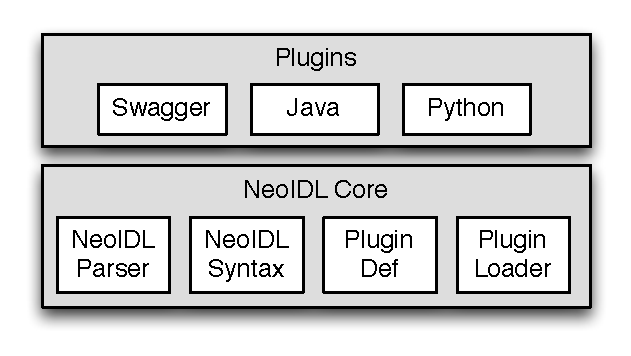
\includegraphics[scale=0.6]{neoidl.pdf}
\vspace{-.5cm}
\end{center}
\caption{Arquitetura do framework de geração de código da \neoidl{}.}
\label{fig:neoidl-architecture} 
\end{figure}


O núcleo do \framework{} possui um uma pequena aplicação que carrega as
definições dos \textit{plugins} e processa os argumentos da chamada do gerador
(o arquivo de contrato que terá o código gerado, o diretório de destino e a
linguagem a ser utilizada). O modo de funcionamento geral do \framework{} é
ilustrado na figura \ref{fig:programGenerator}. O \textit{parser} da \neoidl{}
foi construído utilizando \bnfc{} \cite{ranta-bnfc:2012} com a linguagem
funcional Haskell.

\begin{figure*}[bt]
\begin{center}
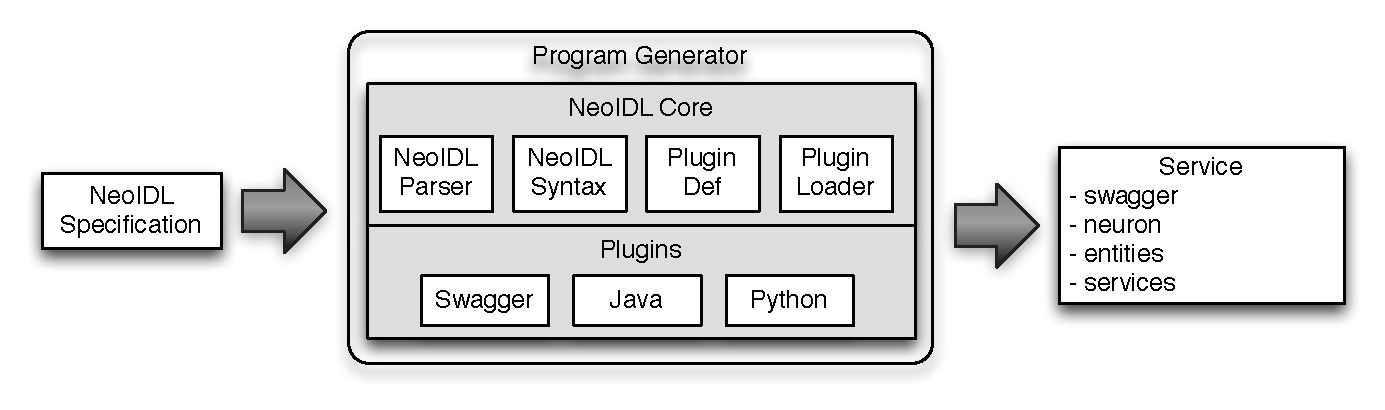
\includegraphics[scale=0.55,trim=0cm 1.5cm 0cm 0cm]{programgenerator.pdf}
\vspace{-.5cm}
\end{center}
\caption{Gerador de código da \neoidl{}}
\label{fig:programGenerator}
\end{figure*}

As próximas subseções detalham o funcionamento de dois módulos onde estão
contidas os principais trechos da lógica implementada na \neoidl{}: O
\textit{PluginDef} e \textit{PluginLoader}.


\subsubsection{Componente PluginDef}{\label{sec:plugindef}}

O desenvolvimento de \textit{plugins} na \neoidl{} devem obedecer algumas regras
de projeto estabelecidas no componente \texttt{PluginDef}, que é um módulo
escrito em Haskell. No \texttt{PluginDef} declara dois tipo de dados
(\texttt{Plugin} and \texttt{GeneratedFile}) e uma assinatura de tipo
(\texttt{Transform = Module -> [GeneratedFile]}). Eles definem uma família de
tipos que mapeiam um módulo \neoidl{} em uma lista de arquivos com o código
gerado ao final do processo.

De acordo com estas regras de projeto, cada \textit{plugin} precisa declarar uma
instância do tipo \texttt{Plugin} e implementar uma função de acordo com a
assinatura definida em \texttt{Transform}. Além disso, cada instância de  
\texttt{Plugin} precisa ter o nome \texttt{plugin} de forma que o componenente
\texttt{PluginLoader} possa obter os dados necessários para o seu processamento.
Assim, a execução de um \textit{plugin} consiste em aplicar sua função de
transformação correspondente a um módulo \neoidl{} e produzir uma lista de
arquivos de código fonte. 

\vspace{6mm}

\begin{figure}[h]
\begin{small}
\lstinputlisting[language=HaskellSimple,firstnumber=1]{pluginDefStructure.tex}
\vspace{-.5cm}
\end{small}
\caption{Assinatura do \texttt{PluginDef}}
\label{lst:pluginDef}
\end{figure}

\subsubsection{Componente PluginLoader}

O carregamento e validação dos \textit{plugins} são competências do componente
\texttt{PlutinLoader}. O primeito passo é listar todos os arquivos do diretório
do \textit{plugin} a ser carregado, filtrar os arquivos Haskell (extensão
\texttt{``.hs''}), criar um nome para um nome reservado (\textit{qualified
name}) para cada arquivo de \textit{plugin} e aplicar a função de compilação.

Caso todas as regras de definição do \textit{plugin} tenham sido atendidas, o
\textit{plugin} é carregado e estará pronto para ser acionado. Caso contrário,
algumas exceções podem ocorrer, como, por exemplo, não haver definição de
nenhum \textit{plugin} no arquivo:

\begin{tabbing}\tt
~\char36{}\char46{}\char47{}neoIDL\\
\tt ~neoIDL\char58{}~panic\char33{}~\char40{}the~\char39{}impossible\char39{}~happened\char41{}\\
\tt ~~\char40{}GHC~version~7\char46{}6\char46{}3~for~x86\char95{}64\char45{}darwin\char41{}\char58{}\\
\tt ~~~~Not~in~scope\char58{}~\char96{}Plugins\char46{}Python\char46{}plugin\char39{}
\end{tabbing}

Ou ainda em razão de o \textit{plugin} não ser uma instância do tipo
\texttt{Plugin}:

\begin{tabbing}\tt
~\char36{}\char46{}\char47{}neoIDL\\
\tt ~neoIDL\char58{}~panic\char33{}~\char40{}the~\char39{}impossible\char39{}~happened\char41{}\\
\tt ~\char40{}GHC~version~7\char46{}6\char46{}3~for~x86\char95{}64\char45{}darwin\char41{}\char58{}\\
\tt ~~Couldn\char39{}t~match~expected~type~\char96{}Plugin\char39{}\\
\tt ~~~with~actual~type~\char96{}\char91{}GHC\char46{}Types\char46{}Char\char93{}\char39{}
\end{tabbing}



\subsection{Linguagem}
\label{linguagemNeoIDL}
\vspace{-6mm}

A \neoidl{} simplifica a especificação de contratos REST pois possui uma sintaxe
concisa própria de linguagens de especificação de interfaces (\emph{interface
description languages}). Ademais, a \neoidl{} provê mecanismos de
modularização e herança, de forma que os contratos possam ser separados em
módulos \footnote{Os arquivos utilizados para definição de contratos
são denominados módulos na \neoidl{}}, facilitando a herança e manutenção dos
contratos.

Para demonstrar como os módulos são estruturados na
\neoidl{}, a seguir são apresentados alguns trechos de um serviço hipotético
de envio de mensagens. Na primeira parte, um módulo faz uma definição de tipo
de dado; em seguida, um segundo módulo, orientado a serviço, importa as
definições do primeiro para então declarar as especificações das operações do
serviço. Por fim, o módulo de serviço é acrescentado de uma anotação como
forma de extender as características da operação.

\vspace{6mm}

\begin{figure}[h]
\begin{small}
\lstinputlisting[language=NeoIDL,firstnumber=1]{mensagemData.tex}
\vspace{-.5cm}
\end{small} 
\caption{Tipos de dados definidos na \neoidl}
\label{lst:messagedata-neo}
\end{figure}

O trecho ilustrado na figura \ref{lst:messagedata-neo} faz a definição de dois
tipos de dados. \emph{MessageType}, declarado no linha 2, é uma estrutura
simples do tipo enumeração. O outro tipo é \emph{Message}, declarado entre as
linhas 4 e 11, composto de seis atributos. O atributo \emph{type} de
\emph{Message} é do tipo \emph{MessageType} recém declarado.

Na \neoidl{} é utiliza a abordagem convenção sobre configuração, de modo que
todos os atributos declarados são obrigatórios, a menos que explicitamente
seja declarado diferente. O atributo \emph{subject} do tipo \emph{Message} é um
exemplo de atributo opcional (\texttt{<Type> <Ident> = 0;}).

O módulo seguinte (figura \ref{lst:sentmessage-neo}), na linha proposta pela
\neoidl{} para suporte a herança e reuso, importa o conjunto de definições de \emph{MessageData} e declara o
serviço \emph{sendbox} (linha 4), o qual possui duas capacidades. A
capacidade \emph{sendMessage} (linha 6) utiliza a operação \method{post} para submeter uma
mensagem (tipo \emph{Message}). A outra capacidade (linha 7) tem a finalidade de
listas as mensagens com um determinado sequecial, por meio da operação
\method{get}.

Por fim, a instrução \emph{path} indica o caminho (URI) onde as
operações serão disponibilizadas. Esse atribuito é importante para se definir
como as requisições serão roteadas entre os serviços.

\vspace{6mm}

\begin{figure}[htb]
\begin{small}
\lstinputlisting[language=NeoIDL,firstnumber=1]{mensagem.tex}
\end{small}
\caption{Sent message service specification in \neoidl}
\label{lst:sentmessage-neo}
\end{figure}

Ainda na filosofia de conversão sobre configuração, a \neoidl{} assume que os
argumentos das operações \method{POST} e \method{PUT} são enviadas no corpo da
requisição. Nas operações \method{GET} e \method{DELETE}, por outro lado,
presume-se que os agumentos estão contidos no \emph{path} da requisição ou ainda
como \textit{query string}.

A especificação dos contratos na \neoidl{} pode ser enriquecida com
anotações, por meio das quais se possibilita extender a semântica de uma
especificação sem que seja necessário alterar a sintaxe da \neoidl{}. Esse
recurso da \neoidl{} simplifica a inclusão de novas características aos
serviços, pois a alteração da sintaxe da própria \neoidl{} envolve um esfoço não
trivial de compatibilizar todos os \textit{plugins} já construídos.

O módulo apresentado na figura \ref{lst:annotationNeoIDL} contém, além das
informações contidas no módulo da figura \ref{lst:sentmessage-neo}, uma anotação chamada
\emph{Security Policy} (linhas 4 a 6) aplicada ao serviço \emph{sentbox}. A
declaração da anotação é feita no final do módulo (linhas 14 a 18).

\vspace{6mm}
 
\begin{figure}
\begin{small}
\lstinputlisting[language=NeoIDL,firstnumber=1]{messageSendAnnotation.tex}
\vspace{-.5cm}
\end{small}
\caption{Especificação de anotação na \neoidl{}}
\label{lst:annotationNeoIDL}
\end{figure}

Além de aplicáveis a \texttt{resources}, as anotações também podem ser aplicadas
a outros construtores da linguagem: \texttt{module}, \texttt{enum},
\texttt{entity}. Qualquer anotação na \neoidl{} possui a mesma estrutura: um
nome, um elemento alvo e uma lista propriedades. Todas estas informações ficam
disponíveis para utilização pelos \textit{plugins}.




\subsubsection{The lexical structure of NeoIDL}\label{sub:lexical}

\begin{enumerate}
  \item Identifiers

Identifiers \nonterminal{Ident} are unquoted strings beginning with a letter,
followed by any combination of letters, digits, and the characters {\tt \_ '},
reserved words excluded.

  \item Literals

String literals \nonterminal{String}\ have the form
\terminal{``}$x$\terminal{``}, where $x$ is any sequence of any characters
except \terminal{``} unless preceded by %% \text{\tt \char92{}}. 

Integer literals \nonterminal{Int}\ are nonempty sequences of digits.

Double-precision float literals \nonterminal{Double}\ have the structure
indicated by the regular expression $\nonterminal{digit}+ \mbox{{\it `.'}} 
\nonterminal{digit}+ (\mbox{{\it `e'}} \mbox{{\it `-'}}? \nonterminal{digit}+)?$ i.e.
two sequences of digits separated by a decimal point, optionally
followed by an unsigned or negative exponent.

  \item Reserved words and symbols
The set of reserved words is the set of terminals appearing in the grammar. 
Those reserved words that consist of non-letter characters are called symbols, 
and they are treated in a different way from those that are similar to identifiers. 
The lexer follows rules familiar from languages like Haskell, C, and Java, including longest match and spacing conventions.

The reserved words used in NeoIDL are the following: \\

\begin{tabular}{lll}
{\reserved{annotation}} &{\reserved{call}} &{\reserved{entity}} \\
{\reserved{enum}} &{\reserved{extends}} &{\reserved{float}} \\
{\reserved{for}} &{\reserved{import}} &{\reserved{int}} \\
{\reserved{module}} &{\reserved{path}} &{\reserved{resource}} \\
{\reserved{string}} & & \\
\end{tabular}\\
  
The symbols used in NeoIDL are the following: \\

\begin{tabular}{lll}
{\symb{\{}} &{\symb{\}}} &{\symb{;}} \\
{\symb{{$=$}}} &{\symb{.}} &{\symb{@}} \\
{\symb{(}} &{\symb{)}} &{\symb{0}} \\
{\symb{{$=$}{$=$}}} &{\symb{{$<$}{$>$}}} &{\symb{{$>$}}} \\
{\symb{{$>$}{$=$}}} &{\symb{{$<$}}} &{\symb{{$<$}{$=$}}} \\
{\symb{[}} &{\symb{]}} &{\symb{@get}} \\
{\symb{@post}} &{\symb{@put}} &{\symb{@delete}} \\
{\symb{/@require}} &{\symb{/@ensure}} &{\symb{/@invariant}} \\
{\symb{/@otherwise}} &{\symb{/**}} &{\symb{*/}} \\
{\symb{*}} &{\symb{@desc}} &{\symb{@param}} \\
{\symb{@consume}} &{\symb{,}} & \\
\end{tabular}\\

\end{enumerate}

\subsubsection{The syntactic structure of NeoIDL}\label{sub:syntactic}

Non-terminals are enclosed between $\langle$ and $\rangle$. 
The symbols  {\arrow}  (production),  {\delimit}  (union) 
and {\emptyP} (empty rule) belong to the following BNF notation.
All other symbols are terminals.\\

\begin{small}
\begin{tabular}{lll}
\label{lst:BNFnot}
{\nonterminal{Modulo}} {\arrow} {\terminal{module}} {\nonterminal{Ident}} {\terminal{\{}} \\ 
 \quad {\nonterminal{ListImport}} \\ 
 \quad {\nonterminal{MPath}} \\ 
 \quad {\nonterminal{ListEnum}} \\ 
 \quad {\nonterminal{ListEntity}} \\ 
 \quad {\nonterminal{ListResource}} \\ 
 \quad {\nonterminal{ListDecAnnotation}} \\ 
{\terminal{\}}}  \\
\end{tabular}\\

\begin{tabular}{lll}
{\nonterminal{Import}} & {\arrow}  &{\terminal{import}} {\nonterminal{NImport}} {\terminal{;}}  \\
\end{tabular}\\

\begin{tabular}{lll}
{\nonterminal{MPath}} & {\arrow}  &{\emptyP} \\
 & {\delimit}  &{\terminal{path}} {\terminal{{$=$}}} {\nonterminal{String}} {\terminal{;}}  \\
\end{tabular}\\

\begin{tabular}{lll}
{\nonterminal{NImport}} & {\arrow}  &{\nonterminal{Ident}}  \\
 & {\delimit}  &{\nonterminal{Ident}} {\terminal{.}} {\nonterminal{NImport}}  \\
\end{tabular}\\

\begin{tabular}{lll}
{\nonterminal{Entity}} & {\arrow}  &{\nonterminal{ListDefAnnotation}} {\terminal{entity}} {\nonterminal{Ident}} {\terminal{\{}} {\nonterminal{ListProperty}} {\terminal{\}}} {\terminal{;}}  \\
 & {\delimit}  &{\nonterminal{ListDefAnnotation}} {\terminal{entity}} {\nonterminal{Ident}} {\terminal{extends}} {\nonterminal{Ident}} {\terminal{\{}} {\nonterminal{ListProperty}} {\terminal{\}}} {\terminal{;}}  \\
\end{tabular}\\

\begin{tabular}{lll}
{\nonterminal{Enum}} & {\arrow}  &{\terminal{enum}} {\nonterminal{Ident}} {\terminal{\{}} {\nonterminal{ListValue}} {\terminal{\}}} {\terminal{;}}  \\
\end{tabular}\\

\begin{tabular}{lll}
{\nonterminal{DecAnnotation}} & {\arrow}  &{\terminal{annotation}} {\nonterminal{Ident}} {\terminal{for}} {\nonterminal{AnnotationType}} {\terminal{\{}} {\nonterminal{ListProperty}} {\terminal{\}}} {\terminal{;}}  \\
\end{tabular}\\

\begin{tabular}{lll}
{\nonterminal{DefAnnotation}} & {\arrow}  &{\terminal{@}} {\nonterminal{Ident}} {\terminal{(}} {\nonterminal{ListAssignment}} {\terminal{)}} {\terminal{;}}  \\
\end{tabular}\\

\begin{tabular}{lll}
{\nonterminal{Parameter}} & {\arrow}  &{\nonterminal{Type}} {\nonterminal{Ident}} {\nonterminal{Modifier}}  \\
\end{tabular}\\

\begin{tabular}{lll}
{\nonterminal{Assignment}} & {\arrow}  &{\nonterminal{Ident}} {\terminal{{$=$}}} {\nonterminal{Value}}  \\
\end{tabular}\\

\begin{tabular}{lll}
{\nonterminal{Modifier}} & {\arrow}  &{\emptyP} \\
 & {\delimit}  &{\terminal{{$=$}}} {\terminal{0}}  \\
\end{tabular}\\

\begin{tabular}{lllllllll}
{\nonterminal{AnnotationType}} & {\arrow}  &{\terminal{resource}}  
 & {\delimit}  &{\terminal{enum}}  
 & {\delimit}  &{\terminal{entity}}  
 & {\delimit}  &{\terminal{module}} 
\end{tabular}\\

\begin{tabular}{lll}
{\nonterminal{Resource}} & {\arrow}  &{\nonterminal{ListDefAnnotation}} {\terminal{resource}} {\nonterminal{Ident}} {\terminal{\{}} {\terminal{path}} {\terminal{{$=$}}} {\nonterminal{String}} {\terminal{;}} {\nonterminal{ListCapacity}} {\terminal{\}}} {\terminal{;}}  \\
\end{tabular}\\

\begin{tabular}{lll}
{\nonterminal{Capacity}} & {\arrow}  &{\nonterminal{NeoDoc}} {\nonterminal{ListDefNAnnotation}} {\nonterminal{Method}} {\nonterminal{Type}} {\nonterminal{Ident}} {\terminal{(}} {\nonterminal{ListParameter}} {\terminal{)}} {\terminal{;}}  \\
\end{tabular}\\


\begin{tabular}{lllllllll}
{\nonterminal{Method}} & {\arrow}  &{\terminal{@get}} 
 & {\delimit}  &{\terminal{@post}} 
 & {\delimit}  &{\terminal{@put}}  
 & {\delimit}  &{\terminal{@delete}} 
\end{tabular}\\
\end{small}    











\section{AVALIAÇÃO EMPÍRICA}
\vspace{-6mm}

% anexar script de transcrição.

\subsection{Expressividade}
\vspace{-6mm}



In Section~\ref{sub:experience} we presented the comparison in SLOC between the contracts
specification in NeoIDL and the resultant code generated by the framework. Another
relevant issue is a comparison of expressiveness of contracts written in \neoidl{} and other popular
languages with the same purpose (specifying contracts for REST services). In this context,
we compared \neoidl{} specifications with Swagger specifications, a language that has been increasily used by the industry.
Swagger ~\cite{swagger} contracts may by written in JSON and Yaml, both based on key-value structure.

In a collaborative work with the Brazilian Army,
we obtained a portion of their contracts' specifications in Swagger (44 in total), specified with version 1.2.
Our first step was to rewrite these specifications in \neoidl{} and thus compare the total
number of lines of code (which might serve as a metric of expressiveness).
The 44 contracts in Swagger amount to 13921 lines of specification, while the same set of contracts in NeoIDL comprises 5140 lines of specification. Thus, the average reduction was about 63\%. In others words, it means that 10 lines of structured Swagger specification require
about 4 lines of \neoidl{} specification. In this analysis we only considered \emph{physical lines of code}, ignoring 
blank lines and lines consisting of delimiters only. The Appendix A shows a sample contract we analised.

The reduction in number of lines is not the same in all contracts. For instance, a given service\footnote{For confidentiality reasons, the real names of contracts were omitted.} required 367 lines of Swagger specification and 112 lines of \neoidl{} specification. This case  
represents a reduction of about 69\%. On the other hand, another service contract required 
81 lines of specification in Swagger and 42 lines of \neoidl{} specification. In this case, the SLOC decrease was slightly less than 50\%.

The size of the original contract has only a small influence in the observed expressiveness. 
Therefore, we cannot assume that \emph{the bigger the contract is in Swagger 
the bigger is the improvement (with respect to the smaller specification size) of \neoidl}. We 
also realized that the use of a more descritive documentation, the number of entities, and the number of capacities do not correlate to the advantageous reduction of lines of code during a 
transformation of Swagger specifications into \neoidl{} specifications. Therefore, it seems that 
the benefits do not relate to the size of the original specifications.  
Table~\ref{tab:size-corr} presents the correlation between the improvement of 
expressiveness (measured as the percentage of reduction obtained 
after transforming Swagger specifications into \neoidl{} specifications) and 
some metrics related to the size of the original Swagger specifications.

\begin{table}[htb]
\caption{Correlation of the Expressiveness Improvement with the size of the Swagger specifications}
\begin{center}
\begin{tabular}{lrr} 
\toprule
Metric & Pearson's correlation & \emph{p-value} \\ \hline \hline 
LOC of Swagger specification & 0.19 &  0.20 \\ 
Number of services & 0.14 & 0.35 \\ 
Number of capacities & 0.14 & 0.34 \\
Number of entities & 0.20 & 0.18 \\ \bottomrule 
\end{tabular} 
\end{center}
\label{tab:size-corr}
\end{table}





\subsection{Potencial de reuso}



Similar to \neoidl{}, Swagger presents 
some mechanisms to reuse user defined structures. Nevertheless, 
this feature is almost ignored in the set of contracts we analysed, which 
leads to the duplication of entities' definition across different 
Swagger specifications. This might have occurred either due to the 
nonintuitive construct for reusing definitions in Swagger (based on 
references to JSON files) and the difficulties to identify 
that one entity had already been specified in another contract.
After analysing the 44 Swagger specifications, we realized that 40 entities 
have been specified in  more than one contract. Actually, one specific 
entity is present in 12 distinct Swagger contracts. 




 
\section{EXTENSÃO DA NEOIDL PARA DESIGN BY CONTRACT}

Influência de Eiffel, JML e Spec\#

Eiffel assertions are Boolean expressions, with a few extensions such as the old
notation. Since the whole power of Boolean expressions is available, they may
include function calls. Because the full power of the language is available to
write these functions, the conditions they express can be quite sophisticated.
\cite{meyer1992applying}

 
 
\subsection{Proposta: Serviços com Desing-by-Contract}
\vspace{-6mm}

Os benefícios esperados pela adoção da arquitetura orientada a serviços
somente serão auferidos com a concepção adequada de cada serviço. 
Por essa razão, é necessário planejar o projeto dos serviços criteriosamente
antes de lançar mão do desenvolvimento, com preocupação especial em garantir
um nível aceitável de estabilidade aos consumidores de cada serviço.
Nessa etapa do projeto de desenho da solução, a especificação do contrato do
serviço (Web API) exerce uma função fundamental. 

Na sociedade civil, contratos são meios de se formalizar acordo entre partes a
fim de definir os direitos e deveres de cada parte e buscar atingir o
objetivo esperado dentro de determinadas regras. Cada parte espera que as outras
cumpram com suas obrigações.
Por outro lado, sabe-se que o descumprimeto das obrigações costuma implicar de
penalizações até o desfazimento do contrato. 

Contratos entre serviços Web seguem em uma linha análoga. O desenho das
capacidades (operações) e dos dados das mensagens correspondem aos
termos do contrato no sentido do que o consumidor deve esperar do serviço
provedor. Porém identificou-se, após ampla pesquisa realizada sobre o tema, que
as linguagens disponíves para especificação de contratos atingem apenas esse
nível de garantias. No contexto de webservices em REST, conforme descrito na
seção \ref{secaoREST}, há ainda a ausência de padrão para especificação
contratos, tal como ocorre com o WSDL adotado em SOAP.

A proposta deste trabalho é extender os níveis de garantias, de modo a promover
um patamar adicional com obrigações mutuas entre os serviços (consumidor e
provedor). Isso se dá para adoção do conceito de Design-by-Contract (debatido
na seção \ref{Design-by-Contract}) em que a execução da
capacidade do serviço garantirá a execução, desde que satisfeitas as condições
prévias. O detalhamento do processo é exposto nas seções que se seguem.

\vspace{-6mm}

\subsubsection{Modelo de operação}
\vspace{-6mm}

As garantias para execução dos serviços são estabelecidas em duas etapas: pré- e
pós-condições. Nas pré-condições o provedor do serviço estabelece os requisitos
para que o serviço possa ser executado. A etapa de pós-condições tem o papel de
validar se a mensagem de retorno do serviço possui resultados válidos.

O diagrama da Figura \ref{FigServiceDbC} descreve como ocorre a operação das
pré- e pós-condições. O processo se inicia com a chamada à capacidade do serviço e a
identificação da existência de uma pré-condição. Caso tenham sido estabelecidas 
pré-condições, essas são avaliadas. Caso alguma delas não tenham sido
satisfeitas, o serviço principal não é processado e o provedor do serviço
retornar o código de falha definido no contrato correspondente.


\begin{figure}[!htb]
\centering
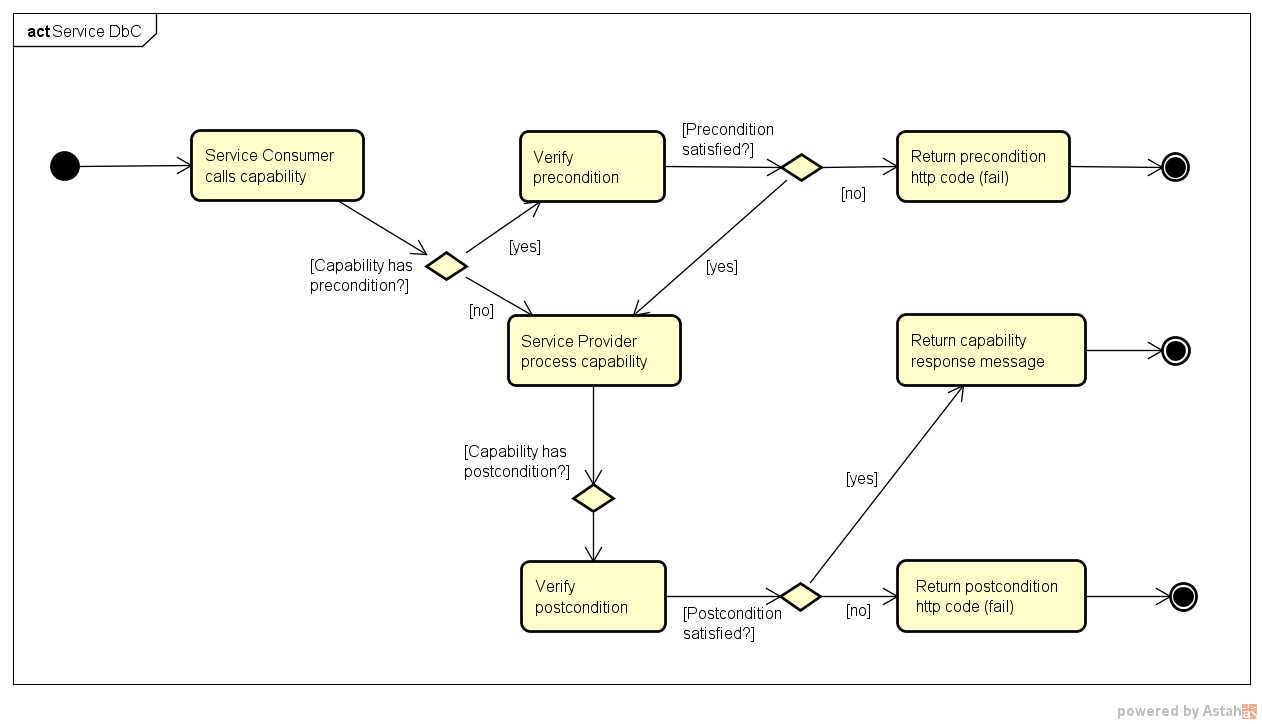
\includegraphics[width=\textwidth,trim = 0mm 5mm 0mm 0mm,clip]{ServiceDbC.png}
\caption{Digrama de atividades com verificação de pré e pós condições}
\label{FigServiceDbC}
\end{figure}

Caso tenham sido definidas pós-condições, essas são acionadas após o
processamento da capacidade, porém antes do retorno ao consumidor do serviço.
Assim, conforme Figura \ref{FigServiceDbC}, visando não entregar ao cliente uma
mensagem ou situação incoerente, as pós-condições são validadas. Caso todas as
pós-condições tenham sido satisfeitas, a mensagem de retorno é encaminhada ao
cliente. Caso contrário, será retornado o código de falha.


\vspace{-6mm}


\subsubsection{Verificação das pré-condições}
\vspace{-6mm}

As pré-condições podem ser do tipo baseado nos parâmetros da requisição ou do
tipo baseado na chamada a outro serviço. Denominamos, para o contexto desta
dissertação, de básica a pré-condição baseada apenas nos parâmetros da
requisição (atributos da chamada ao serviço). Nessa validação é direta,
comparando os valores passados com os valores admitidos. 

No caso das pré-condições baseadas em serviços, é realizada chamada a outro
serviço para verificar se uma determinada condição é satisfeita. Este modo de
funcionamento, que se assemelha a uma composição de serviço, é mais versátil, pois permite
validações de condições complexas sem que a lógica associada seja conhecida pelo
cliente. Assim, os contratos que estabelecem esse tipo de
pré-condição se mantem simples.

A Figura \ref{FigServicePrecondition} detalha as etapas de verificação de cada
pré-condição. Nota-se que a saída para as situações de desatendimento às
pré-condições, independentemente do tipo, é o mesmo. O objetivo desta abordagem
é simplificar o tratametno de exceção no consumidor.

\begin{figure}[!htb]
\centering
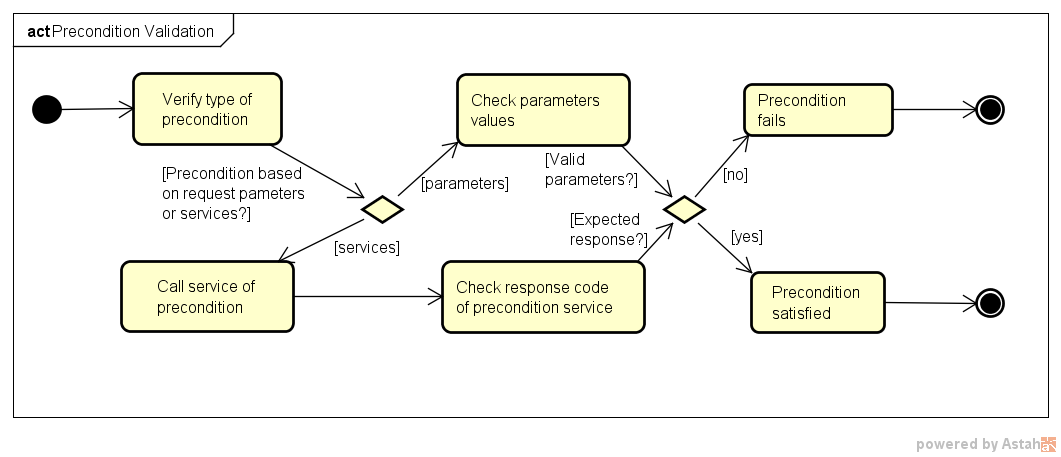
\includegraphics[width=\textwidth,trim = 0mm 5mm 0mm 0mm,clip]{PreconditionValidation.png}
\caption{Diagrama de atividades do processamento da pré-condição}
\label{FigServicePrecondition}
\end{figure}


\subsubsection{Verificação das pós-condições}
\vspace{-6mm}

\begin{figure}[!htb]
\centering
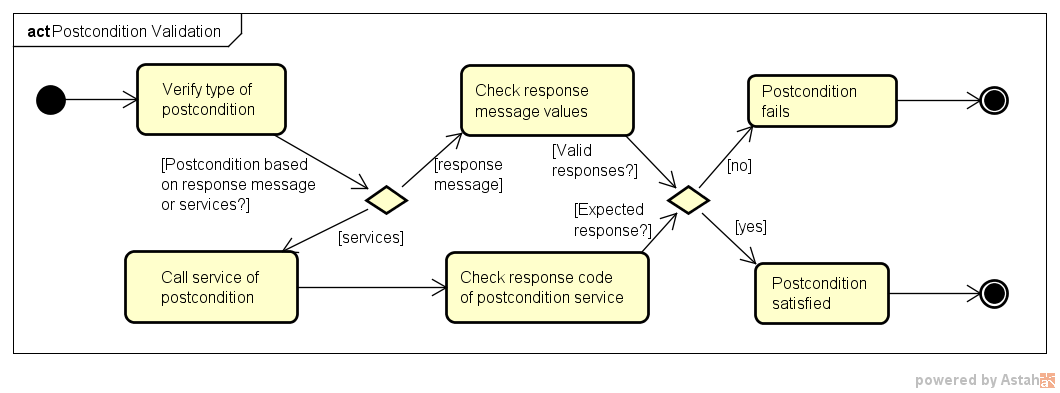
\includegraphics[width=\textwidth,trim = 0mm 5mm 0mm
0mm,clip]{PostconditionValidation.png} 
\vspace{-6mm}
\caption{Diagrama de atividades do processamento da pós-condição}
\label{FigServicePostcondition}
\end{figure}

A verificação das pós-condições acontece de modo muito similar a das
pré-condições. Há também os dois tipos, baseado em valores e em chamadas a
outros serviços. O diferencial está em que a validação dos valores passa a
ocorrer a partir dos valores contidos na mensagem de retorno. A Figura
\ref{FigServicePostcondition} descreve as etapas necessárias para validação de
cada pré-condição.

	
	
	
	

\subsection{Extensão da linguagem}

\subsubsection{Precondição básica}

\begin{figure}[htb]
\begin{small}
\lstinputlisting[language=NeoIDL,firstnumber=1]{DBCsimple.neo}
\end{small}
\caption{Exemplo da notação DBC básica na \neoidl{}}
\label{lst:DBCService}
\end{figure} 

\subsubsection{Pós-condição básica}

\ldots



\subsubsection{Precondição com chamada a serviço}

\begin{figure}[htb]
\begin{small}
\lstinputlisting[language=NeoIDL,firstnumber=1]{DBCservice.neo}
\end{small}
\caption{Exemplo da notação DBC na \neoidl{} com chamada a serviço}
\label{lst:DBCService}
\end{figure} 


\subsubsection{Pós-condição com chamada a serviço}

\ldots

\subsection{Estudo de caso: plugin twisted}

\ldots

\subsubsection{Arquitetura}

% Diagrama da estrutura do código gerado


\subsubsection{Geração de código}